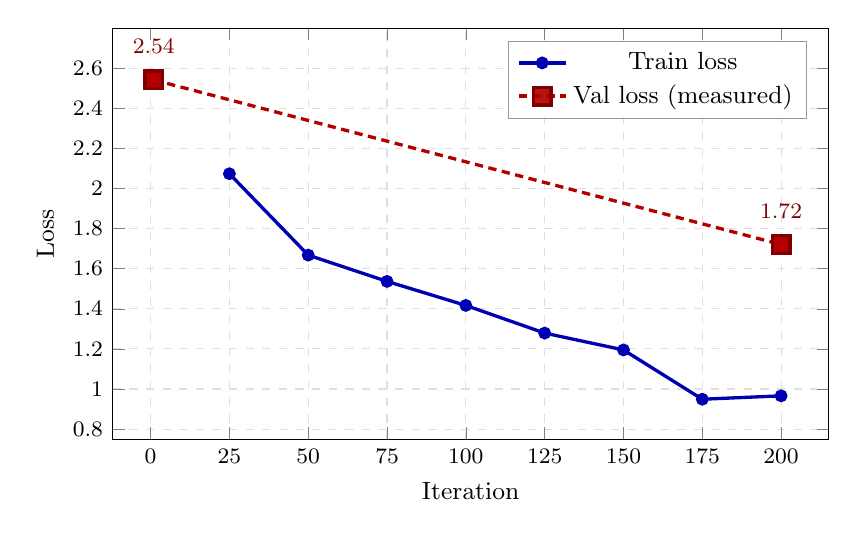
\begin{tikzpicture}
\begin{axis}[
    width=0.88\linewidth,
    height=6.8cm,
    xlabel={Iteration},
    ylabel={Loss},
    xmin=-12, xmax=215,
    ymin=0.75, ymax=2.8,
    xtick={0,25,50,75,100,125,150,175,200},
    ytick={0.8,1.0,1.2,1.4,1.6,1.8,2.0,2.2,2.4,2.6},
    grid=major,
    grid style={dashed,gray!25},
    legend pos=north east,
    legend style={font=\small,fill=white,fill opacity=0.92,text opacity=1,draw=black!40},
    every axis plot/.append style={very thick},
    tick label style={font=\footnotesize},
    label style={font=\small},
    clip=false,
  ]

  % training loss (logged every 25 iters)
  \addplot[
    color=blue!70!black,
    mark=*,
    mark size=1.7pt,
  ] coordinates {
    (25,2.074)
    (50,1.668)
    (75,1.537)
    (100,1.417)
    (125,1.279)
    (150,1.195)
    (175,0.949)
    (200,0.966)
  };
  \addlegendentry{Train loss}

  % validation loss: only measured at iter 1 and iter 200, but rendered
  % with a dashed connecting line for visual continuity.
  \addplot[
    color=red!70!black,
    densely dashed,
    mark=square*,
    mark size=3.2pt,
    mark options={fill=red!70!black, draw=red!50!black, solid},
  ] coordinates {
    (1,2.542)
    (200,1.721)
  };
  \addlegendentry{Val loss (measured)}

  % value labels next to the val markers so they're self-explanatory
  % (yshift pushes labels away from markers for breathing room)
  \node[anchor=south, font=\footnotesize, color=red!50!black, yshift=6pt]
    at (axis cs:1,2.542) {2.54};
  \node[anchor=south, font=\footnotesize, color=red!50!black, yshift=6pt]
    at (axis cs:200,1.721) {1.72};

\end{axis}
\end{tikzpicture}
